\section{Introducing differentiable binary arithmetic operations}
\label{sec:Nalu}
Our goal is to achieve arithmetic operations between the elements of a vector. Such that the output is an addition, subtraction, multiplication, or division of arbitrary elements of a vector $\mathbf{x}$ (e.g. ${x_5 + x_1 \cdot x_7}$), which we formalize as
\begin{equation}
x_1\circ_1 x_2 \circ_2 \cdots x_{k-1} \circ_{k-1} x_{k}\ |\ x_1, x_2, \dots, x_k \in \mathbf{x}, \mathbf{x} \in \mathbb{R}^n, \circ_i \in \{+, -, \times, \div \}.
\label{eq:goal}
\end{equation}
The Neural Arithmetic Logic Unit (NALU) \cite{trask-nalu} attempts to solve problem \ref{eq:goal} by introducing two sub-units; the $\text{NAC}_{+}$ and $\text{NAC}_{\bullet}$ to exclusively represent either the $\{+, -\}$ or the $\{\times, \div \}$ operations.
The NALU attempts to have either $\text{NAC}_{+}$ or $\text{NAC}_{\bullet}$ selected exclusively, which could require the NALU to be applied multiple times (alternating between $\text{NAC}_{+}$ and $\text{NAC}_{\bullet}$) in order to represent the entire space of solutions for equation \ref{eq:goal}.

The $\text{NAC}_{+}$ and $\text{NAC}_{\bullet}$ are defined accordingly,
\begin{align}
W_{h_\ell, h_{\ell-1}} &= \tanh(\hat{W}_{h_\ell, h_{\ell-1}}) \sigma(\hat{M}_{h_\ell, h_{\ell-1}}) \label{eq:weight}\\
\textrm{NAC}_+:\ z_{h_\ell} &= \sum_{h_{\ell-1}=1}^{H_{\ell-1}} W_{h_{\ell}, h_{\ell-1}} z_{h_{\ell-1}} \label{eq:naca}\\
\textrm{NAC}_\bullet:\ z_{h_\ell} &= \exp\left(\sum_{h_{\ell-1}=1}^{H_{\ell-1}} W_{h_{\ell}, h_{\ell-1}} \label{eq:nacm}\log(|z_{h_{\ell-1}}| + \epsilon) \right)
\end{align}
where $\hat{\mathbf{W}}, \hat{\mathbf{M}} \in \mathbb{R}^{H_{\ell} \times H_{\ell-1}}$ are trainable weight matrices, $z_{h_{\ell-1}}$ is the input of size $H_{\ell-1}$, and $H_{\ell}$ is the output size. The matrices are combined using tanh and sigmoid transformation to bias the parameters towards a $\{-1,0,1\}$ solution. Having $\{-1,0,1\}$ allows a linear layer to exactly emulate the binary $\{+, -\}$ operation between elements of a vector as used when computing the $\text{NAC}_{+}$.
The $\text{NAC}_{\bullet}$ extends the $\text{NAC}_{+}$ by using an exponential log transformation, which, with $\{-1,0,1\}$ weight values, becomes the $\{\times, \div \}$ operations (within $\epsilon$ precision).

The NALU combines these units with a gating mechanism $\mathbf{z} = \mathbf{g} \odot \text{NAC}_{+} + (1 - \mathbf{g}) \odot \text{NAC}_{\bullet}$ given $\mathbf{g} = \sigma(\mathbf{G} \mathbf{x})$. The idea is that the NALU should be a plug-and-play component in a neural network and has the ability to, with stochastic gradient descent and backpropagation, to learn the functionality in equation \ref{eq:goal}.

\subsection{Challenges of the $\text{NAC}_{+}$ and $\text{NAC}_{\bullet}$}
To simplify the problem we have chosen to leave out the gating mechanism and focus on the sub-units, assuming "oracle gating". We have not had any consistent success of convergence using the gating mechanism using the NALU or by combining our own proposed sub-units (NAU, NMU), as shown in table \ref{tab:function-task-static-defaults}. We find that gating between $\text{NAC}_{+}$ and $\text{NAC}_{\bullet}$ is challenging. This is likely due to the vastly different gradients, causing addition to be learned much faster than multiplication.

%In section \ref{sssec:weight} we analyse the gradients of equation \ref{eq:weight} and propose a cliped linear alternative, with a regularizer that biases towards $\{-1, 0, 1\}$. This results in an alternative addition unit called NAU.

%In section \ref{sssec:nac-mul} we analyse the gradient of $\text{NAC}_{\bullet}$, and propose an alternative construction called NMU, that has a more well-behaved loss space.

%In section \ref{sssec:nac-add-moments} we analyse the moments of $\text{NAC}_{+}$ and NAU, and derive the optimal weight initializations.

%In section \ref{sssec:nac-mul-moments} we analyse the moments of $\text{NAC}_{\bullet}$ and NMU, and show that the NMU have a more well-behaved expectation and variance. \todo{Maybe remove this overview?}

\subsubsection{Weight matrix construction}\label{sssec:weight}

The weight matrix construction $\tanh(\hat{W}_{h_{\ell-1},h_\ell}) \sigma(\hat{M}_{h_{\ell-1},h_\ell})$ has the properties that could make convergence challenging using gradient decent. Firstly, the gradient of the loss function, $\mathcal{L}$, with respect to the weight matrices, $\hat{W}_{h_{\ell-1},h_\ell}$ and $\hat{M}_{h_{\ell-1},h_\ell}$, can be derived from equation \ref{eq:weight} (derivation in appendix \ref{sec:appendix:gradient-derivatives:weight-matrix-construction}).
\begin{equation}
\begin{aligned}
\frac{\partial \mathcal{L}}{\partial \hat{W}_{h_{\ell-1},h_\ell}} &= \frac{\partial \mathcal{L}}{\partial W_{h_{\ell-1},h_\ell}} (1 - \tanh^2(\hat{W}_{h_{\ell-1},h_\ell})) \sigma(\hat{M}_{h_{\ell-1},h_\ell}) \\
\frac{\partial \mathcal{L}}{\partial \hat{M}_{h_{\ell-1},h_\ell}} &= \frac{\partial \mathcal{L}}{\partial W_{h_{\ell-1},h_\ell}} \tanh(\hat{W}_{h_{\ell-1},h_\ell}) \sigma(\hat{M}_{h_{\ell-1},h_\ell}) (1 - \sigma(\hat{M}_{h_{\ell-1},h_\ell}))
\end{aligned}
\label{eq:nac-weight-gradient}
\end{equation}

For $E[\hat{W}_{h_{\ell-1},h_\ell}] = 0$, which is necessary to satisfy $E[z_{h_\ell}]  = 0$ that is a desired property  \cite{glorot-initialization}, the expectation of the $\hat{M}_{h_{\ell-1},h_\ell}$ gradient becomes zero.

Secondly, in our empirical analysis (see table \ref{tab:function-task-static-defaults}) we find that equation \ref{eq:weight} does not create the desired bias for $\{-1, 0, 1\}$ for the addition and subtraction problem.

To create the desired bias of $\{-1, 0, 1\}$ we add a biasing regularizer $\mathcal{R}_{\ell,\mathrm{bias}}$. To prevent the gradient challenges when $E[\hat{W}_{h_{\ell-1},h_\ell}] = 0$ we propose a simple clamped linear construction with an out-of-bound regularizer $\mathcal{R}_{\ell,\mathrm{oob}}$ to force $\hat{W}$ to be within $[-1, 1]$ and ensure that the gradient is always present. These regualizers are added to the loss function, $\mathcal{L} = \hat{\mathcal{L}} + \lambda_{\mathrm{bias}} \mathcal{R}_{\ell,\mathrm{bias}} + \lambda_{\mathrm{oob}} \mathcal{R}_{\ell,\mathrm{oob}}$.
\begin{align}
W_{h_{\ell-1},h_\ell} &= \min(\max(\hat{W}_{h_{\ell-1},h_\ell}, -1), 1), \\
\mathcal{R}_{\ell,\mathrm{bias}} &= \frac{1}{H_\ell \cdot H_{\ell-1}} \sum_{h_\ell=1}^{H_\ell} \sum_{h_{\ell-1}=1}^{H_{\ell-1}} \hat{W}_{h_{\ell-1},h_\ell}^2 (1 - |\hat{W}_{h_{\ell-1},h_\ell}|)^2 \\
\mathcal{R}_{\ell,\mathrm{oob}} &= \frac{1}{H_\ell \cdot H_{\ell-1}} \sum_{h_\ell=1}^{H_\ell} \sum_{h_{\ell-1}=1}^{H_{\ell-1}} \max(|\hat{W}_{h_{\ell-1},h_\ell}| - 1, 0)^2 \\
\textrm{NAU}:\ z_{h_\ell} &= \sum_{h_{\ell-1}=1}^{H_{\ell-1}} W_{h_{\ell}, h_{\ell-1}} z_{h_{\ell-1}}
\end{align}

\subsubsection{Challenges of division} \label{sssec:nac-mul}

The $\text{NAC}_{\bullet}$, as formulated in equation \ref{eq:nacm}, has the ability to learn exact multiplication and division of elements from a vector if the weights of $W_{h_{\ell-1},h_\ell}$ are one of $\{-1, 0, 1\}$.

However, backpropagation through the $\text{NAC}_{\bullet}$ unit (equation \ref{eq:dz}, derivation in Appendix \ref{sec:appendix:gradient-derivatives:gradient-nac-mul}) reveals that if $|z_{h_{\ell-1}}|$ is near zero, $W_{h_{\ell-1},h_\ell}$ is negative and $\epsilon$ is small, the gradient term will explode and oscillate between large positive and large negative values, which can be problematic in optimization \cite{adam-optimization}, as visualized in figure \ref{fig:nac-mul-eps-issue}.
\begin{align}
%\frac{\partial \mathcal{L}}{\partial W_{h_{\ell}, h_{\ell - 1}}} &= \frac{\partial \mathcal{L}}{\partial z_{h_\ell}} \frac{\partial z_{h_\ell}}{\partial W_{h_{\ell}, h_{\ell - 1}}} = \frac{\partial \mathcal{L}}{\partial z_{h_\ell}} z_{h_\ell} \log(|z_{h_{\ell-1}}| + \epsilon) \label{eq:dw}\\
\frac{\partial \mathcal{L}}{\partial z_{h_{\ell-1}}} &= \sum_{h_\ell = 1}^{H_\ell} \frac{\partial \mathcal{L}}{\partial z_{h_\ell}} \frac{\partial z_{h_\ell}}{\partial z_{h_{\ell-1}}} = \sum_{h_\ell = 1}^{H_\ell} \frac{\partial \mathcal{L}}{\partial z_{h_\ell}} z_{h_\ell} W_{h_\ell, h_{\ell-1}} \frac{\mathrm{sign}(z_{h_{\ell-1}})}{|z_{h_{\ell-1}}| + \epsilon}\label{eq:dz}
\end{align}

This is not an issue for positive values of $W_{h_{\ell-1},h_\ell}$ (multiplication), as $z_{h_{\ell}}$ and $z_{h_{\ell-1}}$ will be correlated causing the terms $z_{h_\ell}$ and $\frac{\mathrm{sign}(z_{h_{\ell-1}})}{|z_{h_{\ell-1}}| + \epsilon}$ to partially cancel out.

This gradient can be particular problematic when considering that $E[z_{h_{\ell-1}}] = 0$ is a desired property when initializing \cite{glorot-initialization}.
A desired multiplication unit should not explode for $z_{h_{\ell-1}}$ near zero, which is why supporting division is likely infeasible.

\begin{figure}[h]
\centering
\begin{subfigure}{.33\textwidth}
  \centering
  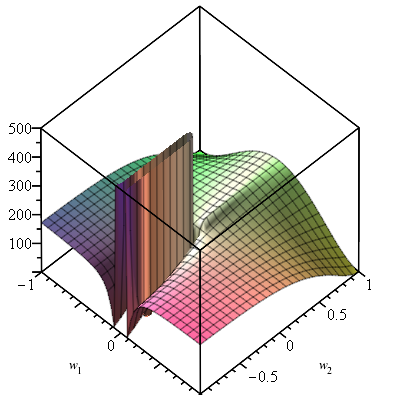
\includegraphics[width=\linewidth]{graphics/nac-mul-eps-1em7.png}
  \caption{$\mathrm{NAC}_{\bullet}$ with $\epsilon = 10^{-7}$}
\end{subfigure}%
\begin{subfigure}{.33\textwidth}
  \centering
  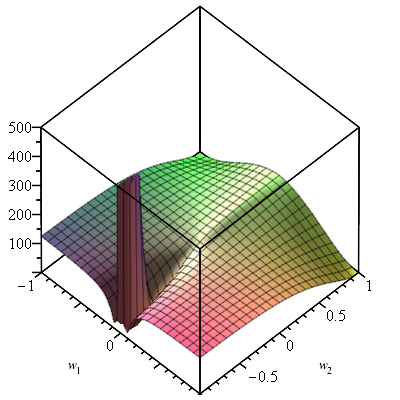
\includegraphics[width=\linewidth]{graphics/nac-mul-eps-1em1.png}
  \caption{$\mathrm{NAC}_{\bullet}$ with $\epsilon = 0.1$}
\end{subfigure}
%\begin{subfigure}{.33\textwidth}
%  \centering
%  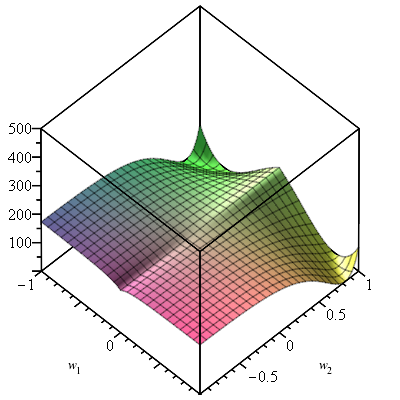
\includegraphics[width=\linewidth]{graphics/nac-mul-eps-1.png}
%  \caption{$\epsilon = 1$}
%\end{subfigure}
\begin{subfigure}{.33\textwidth}
  \centering
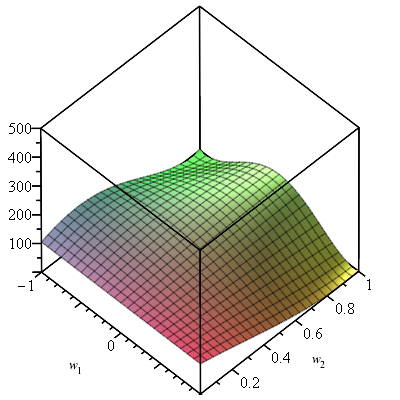
\includegraphics[width=\linewidth]{graphics/nac-mul-nmu.png}
  \caption{Our NMU solution}
\end{subfigure}

\caption{RMS loss curvature for a $\mathrm{NAC}_{+}$ layer followed by either a $\mathrm{NAC}_{\bullet}$ or NMU layer. The weight matrices constrained are to $\mathbf{W}_1 = \left[\protect\begin{smallmatrix}
w_1 & w_1 & 0 & 0 \\
w_1 & w_1 & w_1 & w_1
\protect\end{smallmatrix}\right]$, $\mathbf{W}_2 = \left[\protect\begin{smallmatrix}
w_2 & w_2
\protect\end{smallmatrix}\right]$. The problem is $x = \left(1, 1.2, 1.8, 2\right), t = 13.2$. The desired solution is $w_1 = w_2 = 1$, although this problem have additional undesired solutions.}
\label{fig:nac-mul-eps-issue}
\end{figure}

\subsubsection{Initialization of $\mathrm{NAC}_{\bullet}$}
Initialization is important to consider for fast and consistent convergence, one desired property is that weights can be initialized such that $E[z_{h_\ell}] = 0$ \cite{glorot-initialization}. Using second order Taylor approximation and assuming all $z_{h_{\ell-1}}$ are uncorrelated, the expectation of $\mathrm{NAC}_{\bullet}$ can be estimated as
\begin{equation}
E[z_{h_\ell}] \approx \left(1 + \frac{1}{2} Var[W_{h_\ell, h_{\ell-1}}] \log(|E[z_{h_{\ell-1}}]| + \epsilon)^2\right)^{H_{\ell-1}} \Rightarrow E[z_{h_\ell}] > 1.
\label{eq:nac-mul:expectation}
\end{equation}
As shown in equation \ref{eq:nac-mul:expectation}, satisfying $E[z_{h_\ell}] = 0$ for $\mathrm{NAC}_{\bullet}$ is likely impossible. The variance can also not be input-independent initialized and is expected to explode (proofs in Appendix \ref{sec:appendix:moments:nac-mul}).

\subsubsection{Neural multiplication unit}
To solve the the gradient and initialization challenges for $\mathrm{NAC}_{\bullet}$ we propose a new neural multiplication unit (NMU):

\begin{align}
W_{h_{\ell-1},h_\ell} &= \min(\max(\hat{W}_{h_{\ell-1},h_\ell}, 0), 1), \\
\mathcal{R}_{\ell,\mathrm{bias}} &= \frac{1}{H_\ell \cdot H_{\ell-1}} \sum_{h_\ell=1}^{H_\ell} \sum_{h_{\ell-1}=1}^{H_{\ell-1}} \hat{W}_{h_{\ell-1},h_\ell}^2 (1 - \hat{W}_{h_{\ell-1},h_\ell})^2 \\
\mathcal{R}_{\ell,\mathrm{oob}} &= \frac{1}{H_\ell \cdot H_{\ell-1}} \sum_{h_\ell=1}^{H_\ell} \sum_{h_{\ell-1}=1}^{H_{\ell-1}} \max\left(\left|\hat{W}_{h_{\ell-1},h_\ell} - \frac{1}{2}\right| - \frac{1}{2}, 0\right)^2 \\
\textrm{NMU}:\ z_{h_\ell} &= \prod_{h_{\ell-1}=1}^{H_{\ell-1}} \left(W_{h_{\ell-1},h_\ell} z_{h_{\ell-1}} + 1 - W_{h_{\ell-1},h_\ell} \right) \label{eq:nmu-defintion}
\end{align}
The NMU is regualized similar to the NAU and has a multiplicative identity when $W_{h_{\ell-1},h_\ell}=0$.
The NMU unit does not support division by design.
Previous experiments using the NALU for division does not work well on division hence very little is lost with this modification \cite{trask-nalu}.
As opposed to the $\mathrm{NAC}_{\bullet}$, the NMU can represent input of both negative and positive $z_{h_{\ell-1}}$ values and is not $\epsilon$ bounded, which allows the NMU to extrapolate inputs that are negative or smaller than $\epsilon$.

The gradients with respect to the weight and input in the NMU are (see details in Appendix \ref{sec:appendix:gradient-derivatives:gradient-nmu}):
\begin{align}
\frac{\partial \mathcal{L}}{\partial W_{h_{\ell}, h_{\ell - 1}}} &= \frac{\partial \mathcal{L}}{\partial z_{h_\ell}} \frac{\partial z_{h_\ell}}{\partial W_{h_{\ell}, h_{\ell - 1}}} = \frac{\partial \mathcal{L}}{\partial z_{h_\ell}} \frac{z_{h_\ell}}{W_{h_{\ell-1},h_\ell} z_{h_{\ell-1}} + 1 - W_{h_{\ell-1},h_\ell}} \left(z_{h_{\ell-1}} - 1\right) \label{eq:nmugrad-1} \\
\frac{\partial \mathcal{L}}{\partial z_{h_{\ell-1}}} &= \sum_{h_\ell = 1}^{H_\ell} \frac{\partial \mathcal{L}}{\partial z_{h_\ell}} \frac{\partial z_{h_\ell}}{\partial z_{h_{\ell-1}}} = \sum_{h_\ell = 1}^{H_\ell} \frac{z_{h_\ell}}{W_{h_{\ell-1},h_\ell} z_{h_{\ell-1}} + 1 - W_{h_{\ell-1},h_\ell}} W_{h_{\ell-1},h_\ell} \label{eq:nmugrad-2}
\end{align}

Note that the fraction in equation \ref{eq:nmugrad-1} and \ref{eq:nmugrad-2} does not explode for $z_{h_{\ell-1}}$ close to zero because the denominator cancels out the term for $h_{\ell-1}$ in $z_{h_\ell}$, as seen in equation \ref{eq:nmu-defintion}.

\subsubsection{Moments and initialization}
Our proposed NAU can be initialized using Glorot initialization as it is a linear layer. The $\mathrm{NAC}_{+}$ unit can also achieve an ideal initialization, although it is less trivial (details in Appendix \ref{sec:appendix:moments:weight-matrix-construction}).

Our proposed NMU is initialized with $E[W_{h_{\ell}, h_{\ell - 1}}] = \nicefrac{1}{2}$. Assuming all $z_{h_{\ell-1}}$ are uncorrelated, and $E[z_{h_{\ell-1}}] = 0$, which is the case for most units, the expectation can be approximated to
\begin{equation}
E[z_{h_\ell}] \approx \left(\frac{1}{2}\right)^{H_{\ell-1}},
\end{equation}
which approaches zero for $H_{\ell-1} \rightarrow \infty$ (details in Appendix \ref{sec:appendix:moments:nmu}). The NMU can, with the assumption that, $Var[z_{h_{\ell-1}}] = 1$ and $H_{\ell-1}$ is large, be initialized optimally with $Var[W_{h_{\ell-1},h_\ell}] = \frac{1}{4}$ (proof in Appendix \ref{sec:appendix:moments:nmu:initialization}). 